\chapter{Creating Models in Opus}
\label{chap:creating-models}
\section{Model Types in Opus}

Opus provides infrastructure to develop, specify, estimate, diagnose and predict with a variety of model types.  The Opus GUI currently supports the creation of several types of models by providing templates that can be copied and configured. More will be added in the future.  These initial types are: 

\squishlist
\item Simple Models
\item Sampling Models
\item Allocation Models
\item Regression Models
\item Choice Models
\item Location Choice Models
\squishend 

\subsection{Simple Models}
%
\label{sec:components-simple-model}
\index{models!opus_core models!simple model}
%
The simplest form of a model in Opus is called, for lack of imagination, Simple Model.  It is about as simple as a model can get: compute a variable and write the results to a dataset.  Here are some examples of what could be done with a simple model:

\squishlist
\item Aging Model: add one to the age of each person, each year
\item Walkability Model: write the result of an expression that evaluates the amount of retail activity within walking distance
\item Redevelopment Potential Model: compute the ratio of improvement to total value for each parcel and write this to the parcel dataset
\squishend

A Simple Model template is available in the Model Manager, and can be copied and configured in order to create a new Simple Model like the examples above. It takes only three arguments in its configuration:

\squishlist
\item Dataset: the Opus Dataset that the result will be written to
\item Outcome Attribute: the name of the attribute on the Dataset that will contain the predicted values
\item Expression: the Opus Expression that computes the result to be assigned to the outcome attribute
\squishend 

\subsection{Sampling Models}
The second type of model template is a Sampling Model.  This generic model takes a probability (a rate), compares it to a random number, and if the random number is larger than the given probability (rate), it assigns the outcome as being chosen.  Some examples will make the use of this model clearer. Say we want to build a household evolution model.  We need to deal with aging, which we can do with a Simple Model.  We also models that predict:

\squishlist
\item Births
\item Deaths
\item Children leaving home as they age
\item Divorces
\item Entering the labor market
\item Retiring
\squishend

For all of these examples -- assuming that we want to base our predictions on expected rates that vary by person or household attributes -- we need a more sophisticated model that we shall call a Sampling Model.  Since we need to assign a tangible outcome rather than a probability, we use a sampling method to assign the outcome in proportion to the probability.  This method is also occasionally referred to as a Monte Carlo Sampling algorithm.

The algorithm is simple.  Let's say we have a probability of a coin toss, heads or tails each having a probability of 0.5.  A sampling model to predict an outcome attribute of Heads, would take the expected probability of a fair coint toss resulting in an outcome of Heads as being 0.5.  We then draw a random number from a univariate distribution between 0 and 1, and compare it to the expected probability. If the random draw is greater than the expected probability, then we set the choice outcome to Heads.  If it is less than 0.5, then we set the choice outcome to Tails.  Since we are drawing from a univariate random distribution between 0 and 1, we would expect that around half of the draws would be less than 0.5 and half would be greater than this value.  Larger numbers of draws will tend to converge towards the expected probability by the law of large numbers.  A very large number of draws should match the expected probability to a very high degree of precision.

To make the model useful for practical applications, we can add a means to apply different probabilities to different subsets of the data.  For example, death rates or birth rates vary by gender, age, and race/ethnicity, and to some extent by income.  We might want to stratify our probabilities by one or more of these attributes, and then use the sampling model to sample outcomes using the expected probabilities for each subgroup.

The Sampling Model takes the following arguments:

\squishlist
\item Outcome Dataset: the name of the dataset to receive the predicted values
\item Outcome Attribute: the name of the attribute to contain the predicted outcomes
\item Probability Dataset: the name of the dataset containing the probabilities
\item Probability Attribute: the name of the attribute containing the probability values (or rates)
\item List of Classification Attributes: attributes of Outcome Dataset that will be used to index different Probabilities (e.g. age and income in household relocation)
\squishend

\subsection{Allocation Models}
%
\label{sec:components-allocation-model}
\index{models!opus_core models!allocation model}
%
Another simple generic model supported in Opus is the Allocation Model, which does not require estimating model parameters.  This model proportionately allocates some aggregate quantity to a smaller unit of analysis using a weight.  This model could be configured, for example, to allocate visitor population estimates, military population, nursing home population, and other quantities to traffic analysis zones for use in the travel model system.  Or it could be used to build up a simplistic incremental land use allocation model (though this would not contain much behavioral content).

The algorithm for this type of model is quite simple.  To create an Allocation Model, we need to specify six arguments:

\squishlist
\item Dataset to contain the new computed variable
\item Name of the new computed variable $Y$, which will be indexed by the ids of the dataset it is being allocated to, $Y_i$.
\item Dataset containing the total quantity to be allocated (this can contain a geographic identifier, and will include a year column).
\item Variable containing the control total to be allocated, $T$
\item Variable containing the (optional) capacity value $C$, indexed as $C_i$
\item Variable containing the weight to use in the allocation $w$, indexed as $w_i$, with a sum across all $i$ as $W$
\squishend

The algorithm is then just:

\begin{equation}
Y_i = min(round(T\frac{w_i}{W}),C_i)
\end{equation}

If a capacity variable is specified, we add an iterative loop, from $m$ to $M$, to allocate any excess above the capacity to other destinations that still have remaining capacity:

\begin{equation}
T^m = sum(round(T\frac{w_i}{W}) - C_i)
\end{equation}

In each iteration, we exclude alternatives where $Y>=C$, and repeat the allocation with the remaining unallocated total:

\begin{equation}
Y^m_i = Y^{m-1}_i + (T_m\frac{w_i}{W})
\end{equation}

We then iterate over $m$ until $T^m = 0$ 

This simple algorithm is fairly versatile, and can be used in two modes: as incremental growth or as total values. If used in incremental mode, it adds the allocated quantity to the existing quantities.  The alternative, total, mode for this model replaces the quantities with the new predicted values.

\subsection{Regression Models}
%
\label{sec:components-regression-model}
\index{models!opus_core models!regression model}


Regression models are available to address problems in which the dependent variable is continuous, and a linear equation can be specified to predict it.  The primary use of this model in a core model in UrbanSim is the prediction of property values.  In the context of predicting property values, the model is referred to as a hedonic regression \cite{waddell-hedonic-1993}, but the Opus regression model is general enough to address any standard multiple regression specification.  Other examples of applications for this basic class of models would be to predict water or energy consumption per household, or parking prices.

The basic form is:

\begin{equation}
Y_i = \alpha + \beta X_i + \epsilon_i
\end{equation}

where $X_i$ is a matrix of explanatory, or independent, variables, and $\beta$ is a vector of estimated parameters.  Opus provides an estimation method using Ordinary Least Squares, and additional estimation methods are available by interfacing Opus with the R statistical package.  For the current discussion, we focus on working with the built-in estimation capacity.

\subsection{Choice Models}
%
\label{sec:components-choice-model}
\index{models!opus_core models!choice model}
%

Many modeling problems do not have a continuous outcome, or dependent variable.  It is common to have modeling problems in which the outcome is the selection of one of a set of possible discrete outcomes, like which mode to take to work, or whether to buy or rent a property.  This class of problem we will refer to as discrete choice situations, and we develop choice models to address them.

Recall from Section \ref{sec:discrete-choice} that the standard multinomial logit model \cite{mcfadden-1974,mcfadden-1981} can be specified as:

\begin{equation}
    P_i = \frac{\mathrm{e}^{V_i}}{\sum_j \mathrm{e}^{V_j}},
\end{equation}
where $j$ is an index over all possible alternatives,
$V_i = \beta\cdot {x}_i$ is a linear-in-parameters
function, $x_i$ is a vector of observed, exogenous, independent
alternative-specific variables that may be interacted with the
characteristics of the agent making the choice,
and $\beta$ is a vector of $k$ coefficients
estimated with the method of maximum likelihood \cite{greene-2002}.

The multinomial logit model is a very robust and widely used model in practical applications in transportation planning, marketing, and many other fields.  It is easy to compute and is therefore fast enough to use on large-scale computational problems such as residential location choice.  For explanatory purposes, we will focus initially on choice problems with small numbers of alternatives, such as the choice to rent or own a house, or the number of vehicles a household will choose to own.

Note that there are limitations to the MNL model, and assumptions a user should be aware of.  The most important of these is the Independence of Irrelevant Alternatives (IIA) property, which implies that adding or eliminating an alternative from a choice set will affect all of the remaining alternatives proportionately.  Stated another way, the relative probabilities of any two alternatives will be unaffected by adding or removing another alternative.  See \cite{train-book-2003} for a thorough introduction to discrete choice modeling using MNL and other choice model specifications.

We now turn to a tutorial for creating models of some of these types using the Opus GUI.  In the following sections, we provide a worked example of creating a new model of each type.  The other model types follow the same pattern in the Opus GUI.


\section{Interactive Estimation and Diagnostics}

{\bf Please note:} the seattle\_parcel sample data used in the following
description is only to demonstrate functionality.  One should not read too
much into the results, since seattle\_parcel is a small subset taken from
the PSRC project datasets to make its size more manageable.  In particular,
estimating models with certain specifications may give peculiar results,
such as SE and t-values equal to \verb|-1.#IND| or \verb|-1.#INF| due to
an insufficient number of observations, collinearity, or outliers in the
data.  Estimation results that include erroneous results such as these
cannot saved or exported to a sql database, or viewed in the OPUS GUI\@.

\subsection{Estimation of a Regression Model}

In this section, we take up the topic of estimating and diagnosing models
interactively, from the command line.  Eventually the functions described
here will be available in the Graphical User Interface, but as of now they
are only available from the interactive command mode.

Assume we want to estimate the real estate price model in the
seattle\_parcel project, which includes submodels to separately specify the
model for each general land use type.  If you are using a computer with the
Windows operating system, open a command shell, and type the following:

\begin{verbatim}
python -i c:\opus\src\urbansim\tools\start_estimation.py -x c:\opus\project_configs\seattle_parcel.xml -m real_estate_price_model
\end{verbatim}

Depending on exactly what the specification is, the result would look something like the lsting below:\\

\begin{verbatim}
(clipped results)
...
    ===============================================

    Estimate regression for submodel 28
    Number of observations: 1155
    R-Squared:             0.0096657786478383297
    Adjusted R-Squared:    0.0079464484024351911
    Suggested |t-value| >  2.6555330204981247
    -----------------------------------------------
    Coeff_names estimate        SE      t-values
      constant   3.14716        0.284388         11.0665
      lnempden  0.0471131       0.014493         3.25074
     lngcdacbd  0.244395        0.089292         2.73703
    ===============================================

    Estimate regression for submodel 30
    Number of observations: 456
    R-Squared:             0.23620022093023421
    Adjusted R-Squared:    0.22253042622652475
    Suggested |t-value| >  2.4743671533372704
    -----------------------------------------------
    Coeff_names estimate        SE      t-values
      constant  -10.6226         31.7798        -0.334255
    hbwavgtmda  -0.0372783      0.0168999       -2.20582
    ln_bldgage  -0.0340602      0.0220903       -1.54186
     ln_invfar  0.266353        0.0347524        7.66431
     lnemp20tw  -0.0295508      0.0280097       -1.05502
     lnemp30da   1.37285         2.38156        0.576451
     lngcdacbd  -0.494537       0.219013        -2.25803
        lnsqft  -0.119418       0.0256662       -4.65272
       lnunits  0.206834        0.0271091        7.62969
    ===============================================

Estimating Real Estate Price Model (from urbansim.models.real_estate_price_model): completed...0.9 sec
\end{verbatim}

Since the model was estimated in interactive mode, using the -i option in the python command to start the estimation, the program remains active after estimation is completed, and additional commands may be directly entered at the python prompt: $>>>$.  Assume that we want to further explore the data in submodel 30 (mixed-use properties).  

One of the first things one might wish to do is to examine the correlation among the variables in a model.  We can do this by using one of the built-in estimator methods, plot\_correlation, with the following command:

\begin{verbatim}
>>> estimator.plot_correlation(30)
\end{verbatim}

The method computes a correlation matrix for the data used in submodel 30 and generates a plot of this correlation, as shown in Figure \ref{fig:correlation30}:

\begin{figure}[htp]
\begin{center}
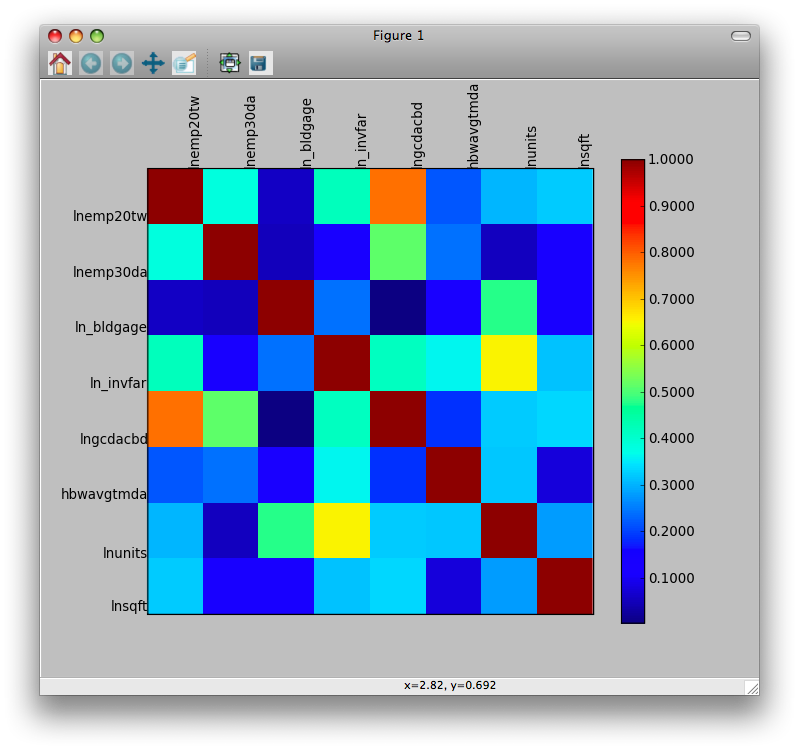
\includegraphics[scale=0.35]{graphics/correlation30.png}
\end{center}
\caption{Correlation Matrix Plot for Submodel 30 in Real Estate Price Modell}
\label{fig:correlation30}
\end{figure}

Note that when a plot is generated from the command line in Python, control of Python is focused on the graphics window, and there is no Python prompt available.  When finished viewing the figure, exit the graphics window by clicking on the x to close it, and the Python prompt will return for more interactive commands.

We can retrieve the data for submodel 30 as a dataset that we can further analyze using Opus methods for the Dataset class.  Begin with the following command to retrieve the data and assign it to an object called ds30 (for submodel 30):

\begin{verbatim}
>>> ds30 = estimator.get_data_as_dataset(30)
>>>
\end{verbatim}

The syntax above indicates that we are executing a method called get\_data\_as\_dataset of the class estimator, which is the class that is running the estimation of the model.  The value 30 in parentheses is an argument being passed to this method, to identify that we want to retrieve only the subset of the data that corresponds with submodel 30.  If we wanted all the data, we would leave out the argument, but keep the empty parentheses.  Note that nothing special happens when this command is executed.  If it succeeded, it will create the new dataset object called ds30, and return to the python prompt.  At this point, we can use a variety of built in methods for the dataset class to further explore the data.  The first of these methods is summary(), which computes a statistical summary of the data in this object, like so:\\

\begin{verbatim}
>>> ds30.summary()
Attribute name	mean       sd	       sum            min             max
-------------------------------------------------------------------------
lnemp20tw       8.96	       1.57     4087.51       5.86363       12.1193
lnemp30da      13.21      0.01     6024.29       13.1266       13.2164
ln_bldgage      3.08        1.41     1404.12      -0.287682    4.60517
ln_invfar       0.23       1.09     104.191       -2.44127     4.56796
lngcdacbd      2.84        0.22     1292.87       2.36556       3.29027
hbwavgtmda     13.15      1.8       5995.99       10.1786       18.0341
lnunits         1.08        1.47     492.089        0            5.63121
lnsqft          9.74        1.17      4440.23       6.42972      14.1835

Size: 456  records
identifiers: 
         id  in range  1 - 456
\end{verbatim}


Another useful Dataset method is the plot\_histogram, which computes a histogram for an attribute of a dataset and plots it, as shown in Figure \ref{fig:histogram-lnsqft}:\\

\begin{verbatim}
>>> ds30 = plot_histogram('lnsqft')
\end{verbatim}

\begin{figure}[htp]
\begin{center}
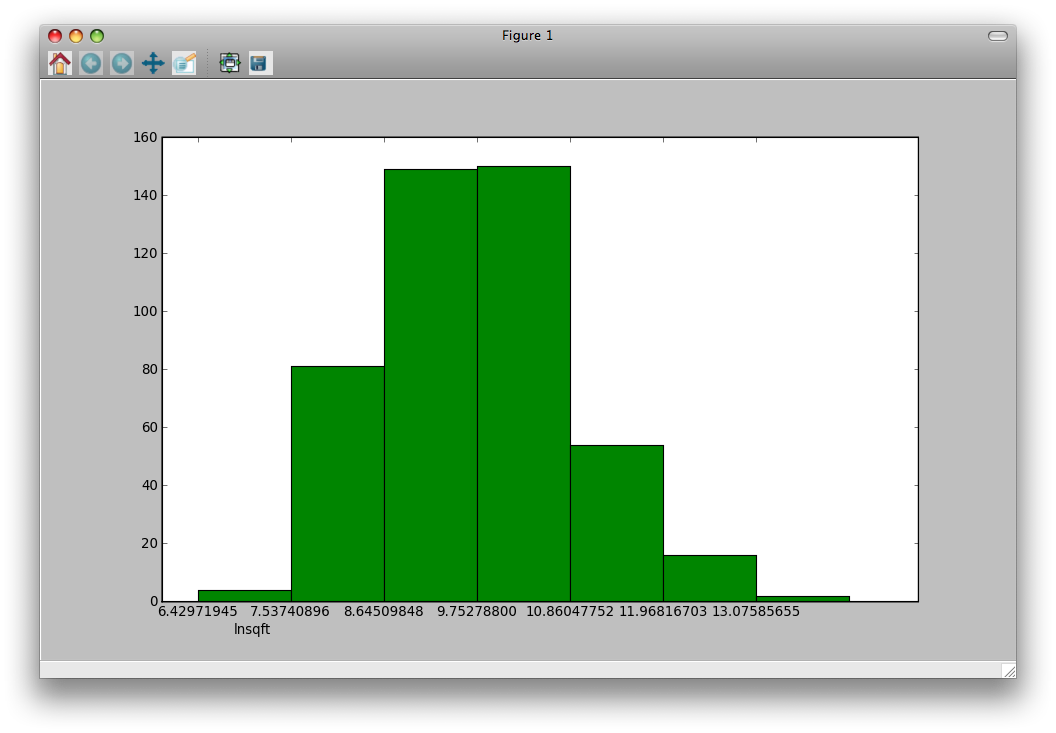
\includegraphics[scale=0.35]{graphics/histogram-lnsqft.png}
\end{center}
\caption{Histogram of Lnsqft from Data in Submodel 30 of the Real Estate Price Modell}
\label{fig:histogram-lnsqft}
\end{figure}


After interactive exploration of the data used in the model, we might choose to drop or add variables from the specification.  For demonstration purposes, drop lnemp30da from the specification of submodel 30, in the GUI, and save the project.  Alternatively this could be done by editing the seattle\_parcel.xml (be careful to use an editor that will not damage the format of the file, for example in Windows you can use a Notepad version that has added XML support). Once the specification has been edited and saved, re-run the estimation for only submodel 30 like this:\\


\begin{verbatim}
>>> estimator.reestimate(30)
Estimating Real Estate Price Model (from urbansim.models.real_estate_price_model): started on Thu May 22 09:36:12 2008
    Estimate regression for submodel 30
    Number of observations: 456
    WARNING: Estimation may led to singularities. Results may be not correct.
    R-Squared:             0.23563241597137002
    Adjusted R-Squared:    0.22368917247092268
    Suggested |t-value| >  2.4743671533372704
    -----------------------------------------------
    Coeff_names estimate        SE      t-values
      constant   7.69055         0.83843         9.17256
    hbwavgtmda  -0.0395769      0.0164105       -2.41168
    ln_bldgage  -0.0340862      0.0220738       -1.54419
     ln_invfar   0.26758        0.0346613        7.71983
     lnemp20tw  -0.030372       0.0279526       -1.08655
     lngcdacbd  -0.545171       0.200477        -2.71937
        lnsqft  -0.118709       0.0256177       -4.63389
       lnunits  0.204933        0.0268876        7.62182
    ===============================================

Estimating Real Estate Price Model (from urbansim.models.real_estate_price_model): completed...0.1 sec
>>> 
>>>
\end{verbatim}

Notice that now we see a warning, indicating a problem in the specification.  Let's drop the least significant variable, lnemp20tw, and try estimating again:

\begin{verbatim}
>>> estimator.reestimate(30)
Estimating Real Estate Price Model (from urbansim.models.real_estate_price_model): started on Thu May 22 09:43:26 2008
    Estimate regression for submodel 30
    Number of observations: 456
    R-Squared:             0.23361810689099238
    Adjusted R-Squared:    0.22337692346414595
    Suggested |t-value| >  2.4743671533372704
    -----------------------------------------------
    Coeff_names estimate        SE      t-values
      constant   6.99788        0.544696         12.8473
    hbwavgtmda  -0.0378939      0.0163405       -2.31901
    ln_bldgage  -0.037881       0.0218001       -1.73765
     ln_invfar  0.271372        0.0344921        7.86765
     lngcdacbd  -0.390517       0.141209        -2.76553
        lnsqft  -0.121596       0.0254847       -4.77133
       lnunits  0.203752        0.0268711        7.58258
    ===============================================
\end{verbatim}

Now the results do not indicate a warning, though we could experiment further to refine the specification. This interactive approach is very efficient for rapidly experimenting with model specifications and re-estimating a single model.  The same approach is available to estimate a subset of the models, using the following syntax:

\begin{verbatim}
>>> estimator.reestimate(submodels=[3,7,9])
\end{verbatim}

\subsection{Estimation of a Choice Model}

From the command shell (but not in python), we can also start the estimation of a choice model, like the housing type choice model created earlier in this chapter:

\begin{verbatim}
python -i c:\opus\src\urbansim\tools\start_estimation.py -x c:\opus\project_configs\seattle_parcel.xml -m housing_type_choice_model 
\end{verbatim}

The resulting output is shown below:

\begin{verbatim}
(clipped listing)
...
            Estimating Choice Model (from opus_core.choice_model): started on Thu May 22 09:51:57 2008
                single_family=(household.disaggregate(building.building_type_id)==19)+1....0.3 sec
                submodel: -2
                Convergence achieved.
                Akaike's Information Criterion (AIC):  333880.22475104179
                Number of Iterations:  18
                ***********************************************
                Log-likelihood is:            -166938.1123755209
                Null Log-likelihood is:       -177492.11908410664
                Likelihood ratio index:       0.059461832801627756
                Adj. likelihood ratio index:  0.059450564695695318
                Number of observations:       256067
                Suggested |t-value| >         3.5289083875852207
                Convergence statistic is:     0.00048567907076085262
                -----------------------------------------------
                Coeff_names     estimate        std err         t-values
                  constant      0.600053        0.00561164        106.93
                    income      1.13913e-05     5.77362e-08      197.299
                ***********************************************
                Elapsed time:  11.355681 seconds
            Estimating Choice Model (from opus_core.choice_model): completed...12.5 sec
        Simulate year 2000: completed...................................14.2 sec
        Closing log file: /Users/pwaddell/opus/data/seattle_parcel/base_year_data/year_2000_log.txt
    Starting simulation for year 2000: completed........................14.4 sec
Start simulation run: completed.........................................14.4 sec
Closing log file: /Users/pwaddell/opus/data/seattle_parcel/base_year_data/run_model_system.log
>>> 
\end{verbatim}

Note that the same method used for the regression model, get\_data\_as\_dataset, can be used to retrieve the data and analyze it interactively. 

%\begin{verbatim}
%# reestimate and analyze data as above
%# in addition
% >>> estimator.plot_choice_set()
% >>> estimator.plot_choice_set_attribute('ln(gridcell.residential_units)')
%
%# if you uncomment line 42 in
%# inprocess/hana/demo/baseline_estimation.py, you can plot the change in
%# utility
% >>> estimator.plot_utility()
%
%# see also python -i urbansim/tools/start_estimation.py --help
%\end{verbatim}
